\documentclass[12pt]{beamer}

% ****************
% ***** INFO *****
% ****************
\usepackage[english]{babel}
\title[]{When the Minimum Wage Really Bites: The Effect of the U.S.-Level Minimum on Puerto Rico}
\subtitle{ECAG-6665: Research Report}
\author[Name Surname]{Alejandro Ouslan}
\institute[institute]{University of Puerto Rico}
\date{} % or \today

% *******************
% ***** PROJECT *****
% *******************
% main color: to black
\definecolor{main}{HTML}{000000}
\setbeamercolor{structure}{fg=main}

% *****************
% ***** THEME *****
% *****************
\usepackage{helvet}
\renewcommand{\familydefault}{\sfdefault}
\setbeamertemplate{frametitle continuation}{\gdef\beamer@frametitle{}}
\setbeamertemplate{footline}{}
\setbeamertemplate{navigation symbols}{}
\usepackage{csquotes}
\usepackage[backend=biber,style=numeric]{biblatex}
\addbibresource{../../reference.bib} % Link to the bibliography file

% *****************
% ***** CODE *****
% *****************
\usepackage{listings}
\lstdefinestyle{py}{
	backgroundcolor=\color{white},
	basicstyle=\ttfamily\scriptsize,
	breaklines=true,
	commentstyle=\color{gray},
	keywordstyle=\color{blue},
	stringstyle=\color{magenta},
	language=Python
}

% **********************
% ***** ALGORITHMS *****
% **********************
\usepackage{algorithm}
\usepackage{algpseudocode}

% *****************
% ***** UTILS *****
% *****************
\usepackage{xcolor}

% ********************
% ***** DOCUMENT *****
% ********************
\begin{document}

% **********************
% ***** TITLEPAGE ******
% **********************
\begin{frame}{}
	\vspace{\fill}

	
\includegraphics[width=0.16\linewidth]{../../assets/uprm_logo.png}

	\vspace{\fill}

	\Large
	\color{main}
	\inserttitle

	\medskip

	\large
	\color{black}
	\insertsubtitle

	\vspace{\fill}

	\footnotesize
	\insertinstitute

	\vspace{\fill}

	\textbf{Author:} \insertauthor

	\medskip

	\insertdate

	\vspace{\fill}
\end{frame}

% *****************
% ***** START *****
% *****************
\begin{frame}[allowframebreaks]{Research Question}
	\begin{itemize}
		\item This research paper look to answer to what extent has the U.S>-level minimum reduce employment in Puerto Rico.\cite{castillo1992minimum}
	\end{itemize}

\end{frame}

\begin{frame}[allowframebreaks]{Justification of Research}
	\begin{itemize}
		\item The mainland U.S. minimum wage was initially applied to Puerto Rico, setting it at \$0.35, which threatened to harm the island's economy.
		\item Recognizing the negative impact, Congress amended the law to establish industry-specific committees in Puerto Rico to set separate minimum wage levels.
		\item Between 1940 and 1974, amendments to the FLSA expanded minimum wage coverage in Puerto Rico, but the industry-committee system remained in place.
	\end{itemize}

\end{frame}

\begin{frame}[allowframebreaks]{Literature Review}
	\begin{itemize}
		\item The U.S.-level minimum altered the distribution of earnings in Puerto Rico to an extraordinary extent, creating marked spikes that dominate
		      the earnings distribution. \cite{brown1988minimum}
		\item Imposing the U.S.-level minimum reduced total island employment by 8-10 percent. \cite{brown1982effect}
		\item Migrants from Puerto Rico to the United States are drawn largely from persons jobless on the island, with characteristics that make them
		      liable to have been disemployed by the minimum wage. \cite{castillo1983jobless}
	\end{itemize}

\end{frame}

\begin{frame}[allowframebreaks]{Data Characteristics and Data Sources}
	\begin{itemize}
		\item The first dataset consits of wage distributions for workers incovered industris obtained fro BLS.
		\item The second dataset is an examination of earnings form the 1980 Census of Pulation for PR.
		\item The third dataset is PR earnings distribution is usal hourly ernings(= usual weekly ernings/usal hours worked) from the CPS in PR.
	\end{itemize}
\end{frame}

\begin{frame}[allowframebreaks]{Methodology}
	\begin{itemize}
		\item The model is a regressed ratio of net migratiants to the PR population (MIG).
		      \begin{equation}
			      \begin{split}
				      MIG = -.14 + \log(USGNP) - .05 \log(PRGNP) + \\
				      .005 \log(MIN) - .17 PRUS
			      \end{split}
		      \end{equation}
	\end{itemize}

\end{frame}

\begin{frame}[allowframebreaks]{Results Figures}
	\begin{center}
		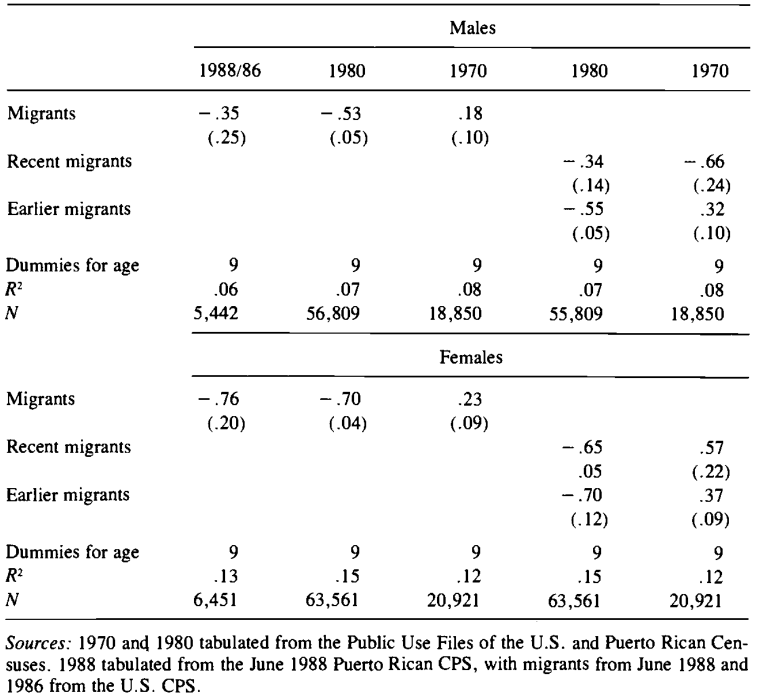
\includegraphics[width=.8\linewidth]{assets/results.png}
	\end{center}
\end{frame}

\begin{frame}[allowframebreaks]{Descriptive Statistics}
	\begin{center}
		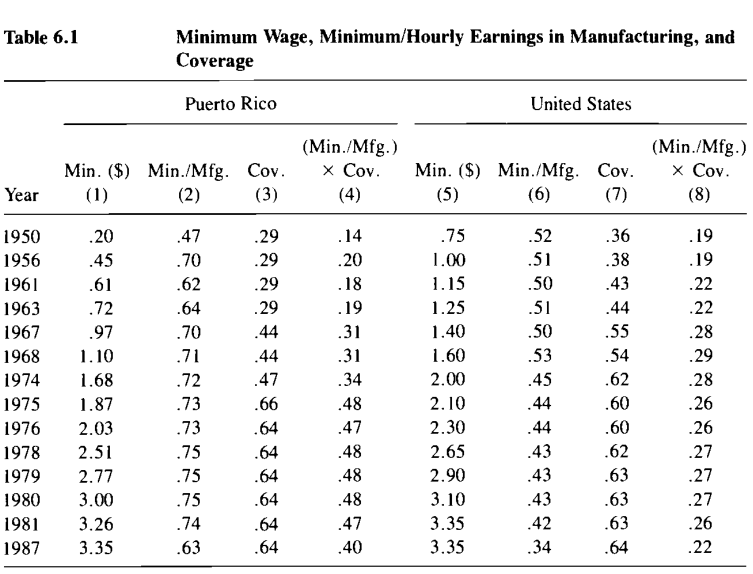
\includegraphics[width=.8\linewidth]{assets/discriptive.png}
	\end{center}
\end{frame}

\begin{frame}[allowframebreaks]{Results}
	\begin{itemize}
		\item If Puerto Ricans of working age living in the U.S. returned to the island, the working-age population would increase by about 50\%.
		\item Assuming 70-80\% of these return migrants would be unemployed with a U.S.-level minimum wage, the unemployment rate would rise to 30-35\%.
		\item The high unemployment rate suggests the U.S.-level minimum wage could not have been applied to Puerto Rico without massive migration.
		\item If migration and the minimum wage had not occurred, labor supply would have increased by 0.40 In points in 1980.
	\end{itemize}
\end{frame}

\begin{frame}[allowframebreaks]{Graphs}
	\begin{center}
		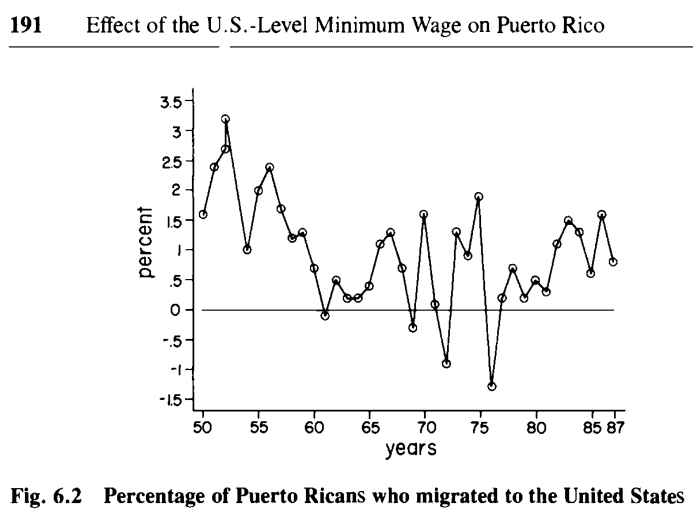
\includegraphics[width=1\linewidth]{assets/graph.png}
	\end{center}
\end{frame}

\begin{frame}[allowframebreaks]{Conclusions}
	\begin{itemize}
		\item The U.S.-level minimum wage distorted Puerto Rico's earnings distribution, reduced employment, and led to labor reallocation across industries.
		\item Without migration, the imposition of the U.S.-level minimum wage would have caused a significant rise in unemployment, challenging the policy's viability.
		\item Migration, particularly of less-skilled workers, was crucial for implementing the U.S. minimum wage and contributed significantly to the growth of real earnings on the island.
		\item The paper highlights the link between domestic labor market policies (like the minimum wage) and migration, emphasizing migration's potential to foster real wage growth in the source economy.
	\end{itemize}
\end{frame}
% ************************
% ***** BIBLIOGRAPHY *****
% ************************
\begin{frame}[allowframebreaks]{Bibliography}
	\printbibliography
\end{frame}
% ***************
% ***** END *****
% ***************

\end{document}
